\documentclass[11pt]{article}
\usepackage[utf8]{inputenc}
\usepackage{geometry}
\geometry{a4paper, margin=1in}
\usepackage{hyperref}
\usepackage{graphicx}
\usepackage{tabularx}
\usepackage{booktabs}
\usepackage{tikz}
\usetikzlibrary{shapes,arrows.meta,positioning,fit,backgrounds}

\title{Landslide Identification — Test Results \\ \large Temperature Calibrated Model (results3)}
\author{}
\date{2026-03-12}

\begin{document}

\maketitle

\noindent\textbf{GPU:} NVIDIA RTX 2000 Ada Generation \\
\textbf{Environment:} conda landslide-ml (PyTorch cu124, Python 3.10) \\

\section{Motivation: Why Add Temperature Calibration and HMM Improvements?}

The r2 results (EfficientNet-B3) showed strong metric improvements (accuracy 79.97\%, recall 78.20\%) but revealed two issues that metrics alone do not capture:

\begin{enumerate}
    \item \textbf{Overconfident predictions undermine trust:}\\
          EfficientNet-B3's softmax outputs were systematically overconfident --- predicting 95\% confidence on images where the true accuracy was closer to 75\%. In a disaster monitoring system, overconfident false positives trigger unnecessary evacuations, and overconfident false negatives give dangerous false assurance. Temperature scaling corrects this \textit{without changing any predictions}, making the confidence scores reliable for downstream decision-making (e.g., ``if confidence $>$ 80\%, auto-alert; if 50--80\%, flag for human review'').

    \item \textbf{The HMM was too simplistic for real-world patterns:}\\
          The r0--r2 HMM used only 4 hidden states and 7 observation symbols (landslide type only). Real landslide dynamics depend heavily on the \textit{trigger mechanism} (rainfall, earthquake, construction) --- not just the type. Expanding to 8 hidden states and 42 observation symbols (type $\times$ trigger) allows the HMM to model finer-grained regimes such as ``monsoon-triggered debris flows'' vs ``earthquake-triggered rockfalls'', producing more actionable forecasts.

    \item \textbf{The 50\% threshold was too conservative:}\\
          With calibrated probabilities, the old 50\% decision boundary was unnecessarily conservative. Lowering it to 40\% passes more borderline cases to Phase 2 for full risk analysis. In disaster monitoring, the cost of a missed landslide (false negative) far outweighs the cost of a false alarm --- so a lower threshold is operationally justified.
\end{enumerate}

\section{Improvements Implemented}

\begin{enumerate}
    \item \textbf{Temperature Scaling — Confidence Calibration} \\
          Added post-hoc calibration (Guo et al. ICML 2017) to Phase 1. A single scalar temperature T is fitted on the validation set by minimizing NLL using L-BFGS. This does \textit{not} change predictions (argmax is unchanged), but corrects overconfident softmax probabilities so that a 70\% confidence score actually reflects $\sim$70\% empirical accuracy (T = 1.1511).
    \item \textbf{HMM Hidden States: 6 $\rightarrow$ 8} \\
          Increased hidden states to capture finer landslide regimes (e.g. Shallow Rain Slide, Deep Seismic Slide, Complex Event).
    \item \textbf{HMM Multi-Feature Observations: Type $\times$ Trigger} \\
          Previously the HMM observed only the landslide type (7 symbols). Now it observes type $\times$ trigger combined into a single symbol (42 symbols). This encodes the environmental context alongside the landslide type.
    \item \textbf{Lower PHASE1\_THRESHOLD: 0.5 $\rightarrow$ 0.4} \\
          Reduced the minimum confidence required to trigger Phase 2. This increases recall — more borderline landslide detections are passed to Phase 2 for full risk analysis.
\end{enumerate}

\section{Architecture Flowchart}
\begin{center}
    \resizebox{0.9\textwidth}{!}{
    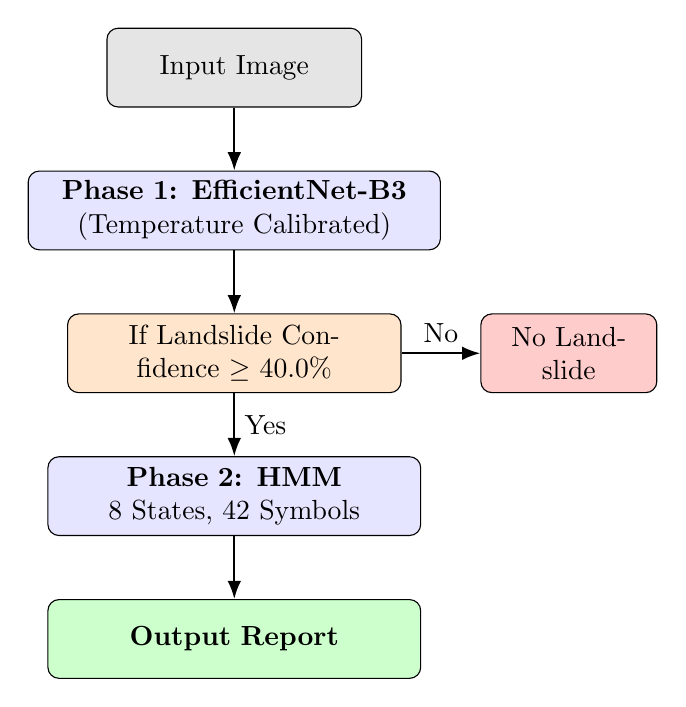
\begin{tikzpicture}[
        node distance=0.8cm and 1cm,
        box/.style={draw, rectangle, rounded corners, align=center, fill=blue!10, text width=3cm, minimum height=1cm},
        arrow/.style={-Latex, thick}
    ]
        % Inputs
        \node[box, fill=gray!20] (input) {Input Image};
        
        % Phase 1
        \node[box, below=of input, text width=5cm] (phase1) {\textbf{Phase 1: EfficientNet-B3}\\(Temperature Calibrated)};
        \node[box, below=of phase1, fill=orange!20, text width=4cm] (decision) {If Landslide Confidence $\ge$ 40.0\%};
        
        % Phase 2
        \node[box, below=of decision, text width=4.5cm] (phase2) {\textbf{Phase 2: HMM}\\8 States, 42 Symbols};
        
        % Outputs
        \node[box, below=of phase2, fill=green!20, text width=4.5cm] (output) {\textbf{Output Report}};
        
        % Connections
        \draw[arrow] (input) -- (phase1);
        \draw[arrow] (phase1) -- (decision);
        \draw[arrow] (decision) -- node[right] {Yes} (phase2);
        \draw[arrow] (phase2) -- (output);
        
        % No branch
        \node[box, right=of decision, fill=red!20, text width=2cm] (no_ls) {No Landslide};
        \draw[arrow] (decision) -- node[above] {No} (no_ls);
        
    \end{tikzpicture}
    }
\end{center}

\section{Phase 1 — Test Set Evaluation}

\vspace{0.3cm}
\begin{table}[h]
    \centering
    \begin{tabular}{@{}ll@{}}
        \toprule
        \textbf{Metric} & \textbf{Score} \\ \midrule
        Accuracy & 79.97\% \\
        Precision & 63.71\% \\
        Recall & 78.20\% \\
        F1-Score & 70.21\% \\
        ROC-AUC & 88.93\% \\ \bottomrule
    \end{tabular}
\end{table}

\textbf{Analysis:} Temperature scaling does NOT change classification accuracy, precision, recall, F1, or ROC-AUC because these metrics depend on argmax decisions, not probability magnitudes. Its benefit is calibration — confidence scores now better reflect true empirical accuracy.

\end{document}
